%!TEX root = ../thesis.tex

%jama -- closed-loop results chapter

\chapter{Closed-Loop Results: MPC-Driven Micro Simulation}
\label{ch:closed_loop}

\section{Simulation Setup}
\label{sec:cl_setup}

%jama
All simulations are run over $T = 150$~days with the parameters described in Chapters~\ref{ch:macro_model} and~\ref{ch:abm}.
Two scenarios are compared:
\begin{enumerate}
  \item \textbf{MPC-controlled scenario}: $\beta_1(t)$ and $\beta_2(t)$ are taken from the Simulink/MPC output.
  \item \textbf{Uncontrolled baseline}: $\beta_1(t) = \beta_2(t) = 0.45$ (the nominal transmission rate) throughout the simulation horizon.
\end{enumerate}
In both scenarios, the micro model is initialised identically (\texttt{rng(1)}, same initial infected and vaccinated agents) to ensure a fair comparison.

The primary outcome measures are:
\begin{itemize}
  \item total infected ($I + I_v$) and hospitalised ($H$) agents as a function of time;
  \item cumulative deaths ($D$) at day 150;
  \item city-level breakdown of infections and hospitalisations;
  \item hospital load relative to capacity.
\end{itemize}
Results below represent single simulation runs; the stochastic nature of the ABM implies that results will vary across runs, and the reported trajectories should be interpreted as representative realisations rather than expected values.

\section{Macro-Level MPC Output}
\label{sec:mpc_output}

%jama
The macro-level MPC controller generates time-varying transmission rates $\beta_1(t)$ and $\beta_2(t)$, which are then used as inputs to the micro agent-based model.
Initially, both transmission rates are reduced from their nominal value as hospital load rises, reflecting the controller's effort to suppress epidemic growth before the healthcare system approaches critical capacity.

Figure~\ref{fig:effective_beta} shows the resulting $\beta(t)$ trajectories over the 150-day horizon.

\begin{figure}[ht]
  \centering
  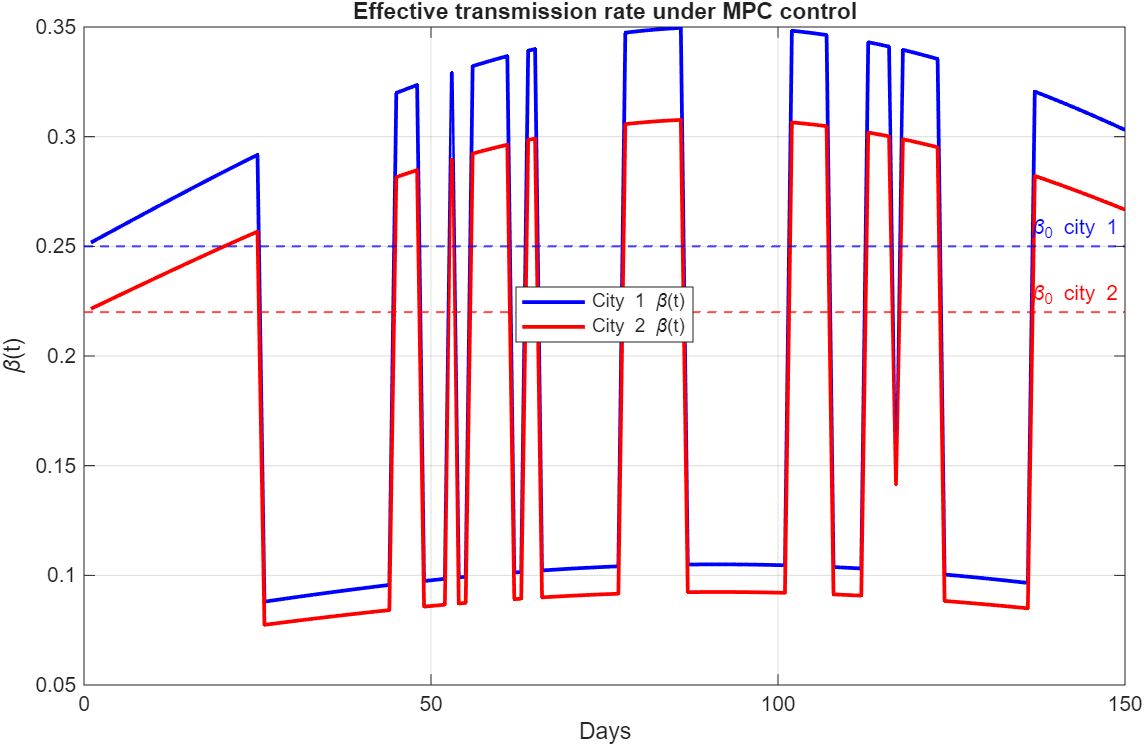
\includegraphics[width=0.85\textwidth]{Figures/jama/effective_beta_uploaded}
  \caption{%jama
    Effective transmission rates $\beta_1(t)$ and $\beta_2(t)$ generated by the
    macro-level MPC controller over 150~days.
    Both cities experience a strong initial reduction in transmission,
    followed by a gradual relaxation as hospital load declines.}
  \label{fig:effective_beta}
\end{figure}

The controller applies the strongest reductions during periods of elevated epidemic pressure and relaxes these reductions as the system stabilises, consistent with the MPC objective of balancing epidemic suppression against the cost of intervention \citep{kohler2021,esterhuizen2024}.

Figure~\ref{fig:intervention_u} shows the corresponding intervention signal $u(t)$.

\begin{figure}[ht]
  \centering
  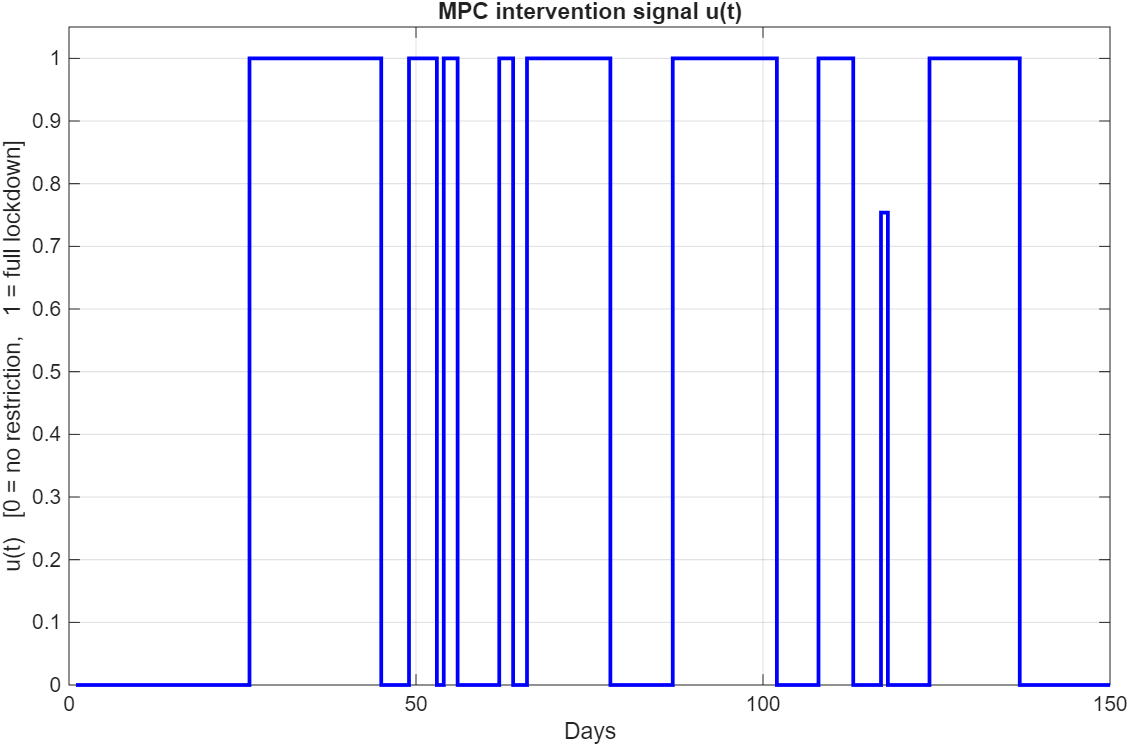
\includegraphics[width=0.85\textwidth]{Figures/jama/mpc_intervention_u_uploaded}
  \caption{%jama
    MPC intervention signal $u(t)$ over the simulation horizon.
    Higher values correspond to stronger non-pharmaceutical interventions
    and larger reductions in the effective transmission rate.
    The controller exhibits a switching-like response, activating strong interventions
    when hospital load approaches the reference threshold.}
  \label{fig:intervention_u}
\end{figure}

\section{MPC-Controlled Scenario}
\label{sec:cl_controlled}

%jama
Under MPC control, the epidemic dynamics are substantially attenuated compared to the uncontrolled baseline.
The controlled results show that infection peaks are reduced and spread over a longer time horizon, while hospitalisation levels remain comparatively stable.
At the same time, the two cities do not evolve identically: small differences in random transmission events and commuting interactions create visible divergence between local trajectories, illustrating why the micro-level model adds value beyond the aggregate macro dynamics.

\section{Uncontrolled Baseline}
\label{sec:cl_uncontrolled}

%jama
In the uncontrolled scenario ($\beta(t) = 0.45$ constant throughout), the epidemic grows rapidly from the initial infected agents.
The infected population rises steeply in the first 30-40 days before plateauing as the susceptible pool is depleted.
Hospital load substantially exceeds the reference threshold, and cumulative deaths are markedly higher than in the MPC-controlled scenario.
This qualitative behaviour is consistent with classical SIR epidemic theory: at $\beta = 0.45$ and $\gamma = 1/12$ the basic reproduction number $R_0 = \beta/\gamma = 5.4$, well above the epidemic threshold \citep{kermack1927,hethcote2000,darienzo2020}.

\section{Comparison and Key Observations}
\label{sec:cl_comparison}

\subsection{Infection Dynamics}
\label{sec:cl_infections}

%jama
Figure~\ref{fig:infected_cl_ol} compares the total number of infected individuals under closed-loop (CL) MPC control and the open-loop (OL) uncontrolled baseline.
Under MPC control, the infection peak is substantially lower and occurs over a broader time interval, indicating that the controller successfully flattens and delays epidemic growth.

\begin{figure}[ht]
  \centering
  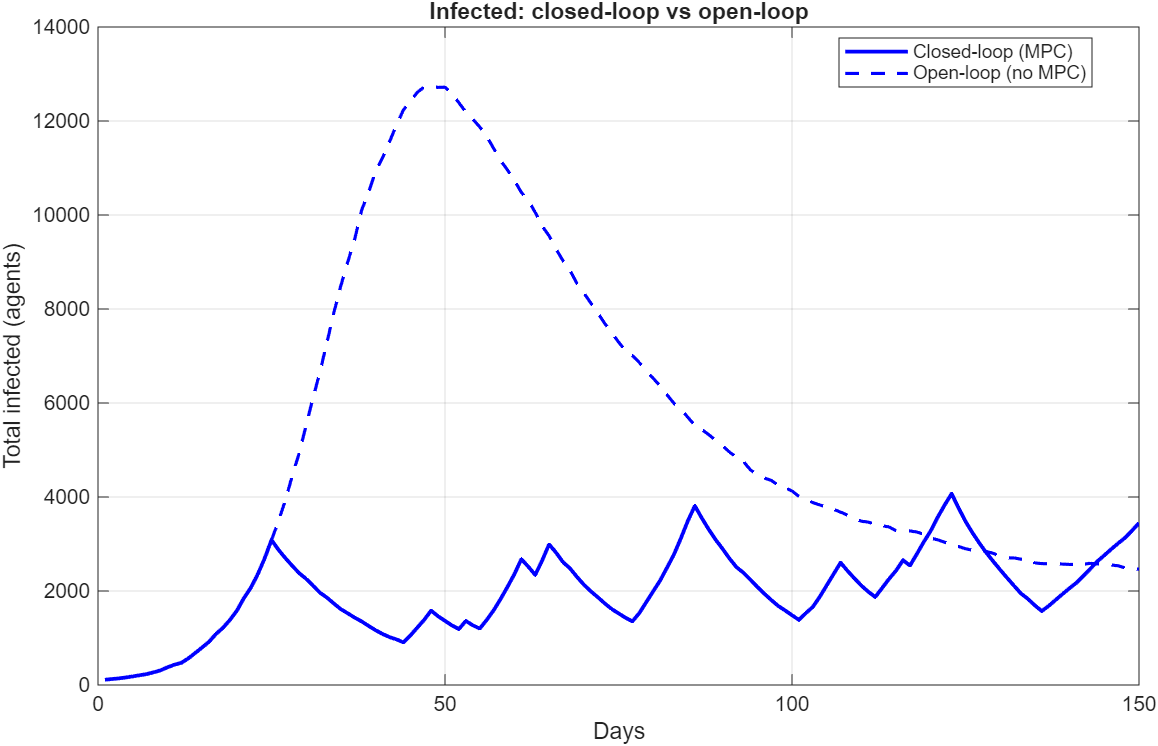
\includegraphics[width=0.85\textwidth]{Figures/jama/infected_cl_vs_ol_uploaded}
  \caption{%jama
    Comparison of total infected individuals under closed-loop (CL) MPC control
    and the uncontrolled open-loop (OL) baseline over 150~days.
    MPC reduces and spreads the infection peak over time.}
  \label{fig:infected_cl_ol}
\end{figure}

\subsection{Hospital Load}
\label{sec:cl_hospital}

%jama
Figure~\ref{fig:hosp_cl_ol} shows the number of hospitalised individuals in the two scenarios.
The uncontrolled baseline produces a much higher and sharper hospitalisation peak, while the controlled case remains more stable and at a significantly lower level.
This demonstrates that reducing transmission through MPC has a direct effect on protecting hospital capacity.

\begin{figure}[ht]
  \centering
  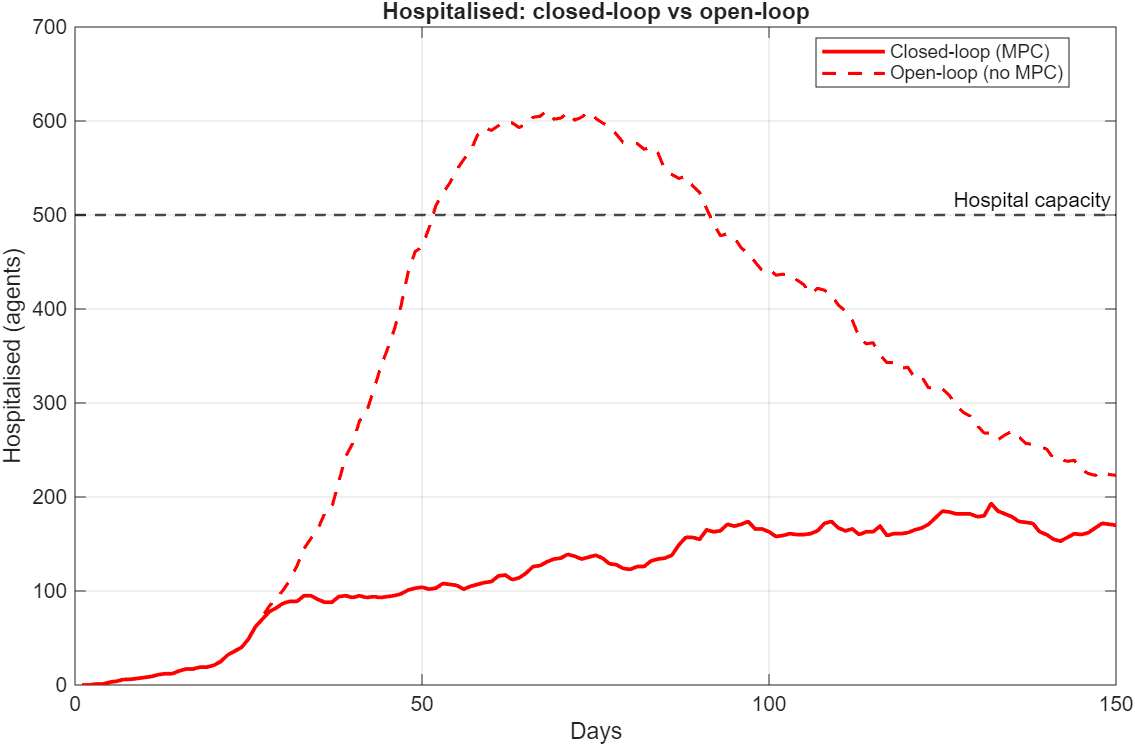
\includegraphics[width=0.85\textwidth]{Figures/jama/hospitalized_cl_vs_ol_uploaded}
  \caption{%jama
    Comparison of hospitalised individuals under closed-loop MPC control
    and the uncontrolled open-loop baseline.
    The controlled scenario keeps hospital occupancy substantially lower throughout.}
  \label{fig:hosp_cl_ol}
\end{figure}

\subsection{Mortality Outcomes}
\label{sec:cl_mortality}

%jama
Figure~\ref{fig:deaths} presents cumulative deaths over the simulation horizon.
The MPC-controlled scenario results in a clear reduction in total mortality compared to the uncontrolled baseline.
This is a direct consequence of limiting infection growth and preventing prolonged periods of high hospital occupancy.

\begin{figure}[ht]
  \centering
  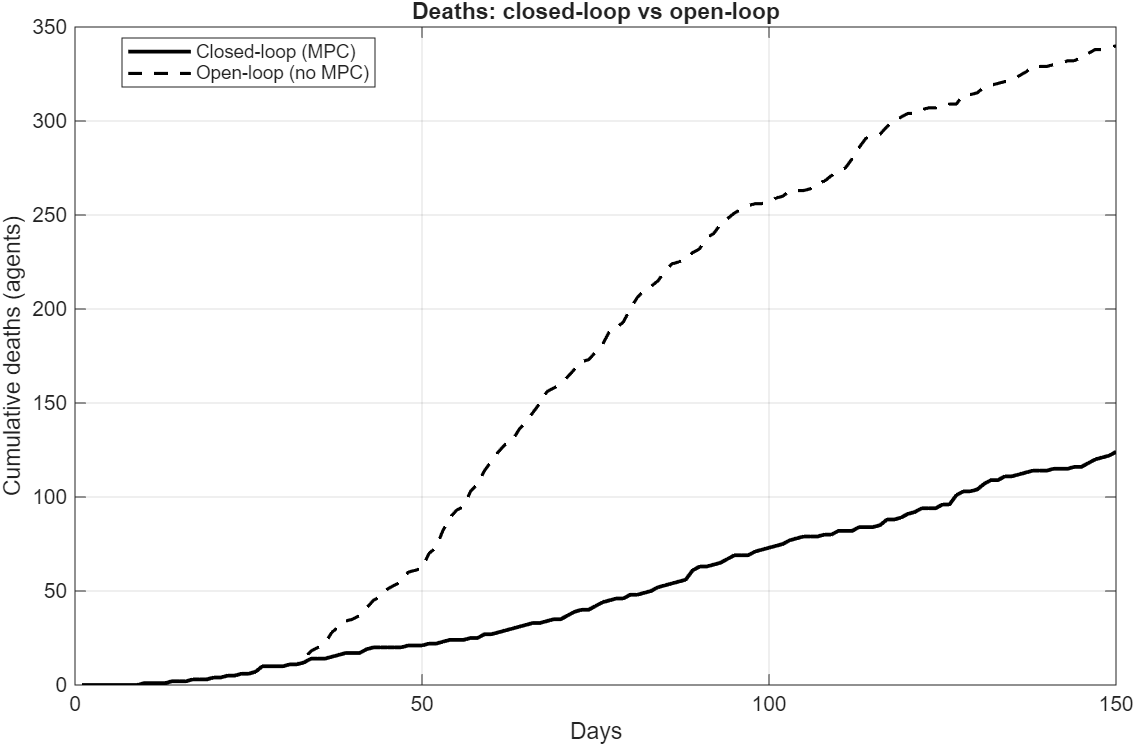
\includegraphics[width=0.85\textwidth]{Figures/jama/deaths_uploaded}
  \caption{%jama
    Cumulative deaths under closed-loop MPC control and the uncontrolled open-loop
    baseline. The controlled scenario yields a substantially lower total death count
    by the end of the 150-day simulation horizon.}
  \label{fig:deaths}
\end{figure}

\subsection{Hospital Capacity Constraint}
\label{sec:cl_capacity}

%jama
Figure~\ref{fig:h_load_vs_ref} compares hospital load in the controlled case with the MPC reference threshold.
The controller keeps the hospital load near or below the target value for most of the simulation horizon, showing that the macro-level constraint-handling objective remains meaningful when the same control signal is applied to the stochastic micro model.

\begin{figure}[ht]
  \centering
  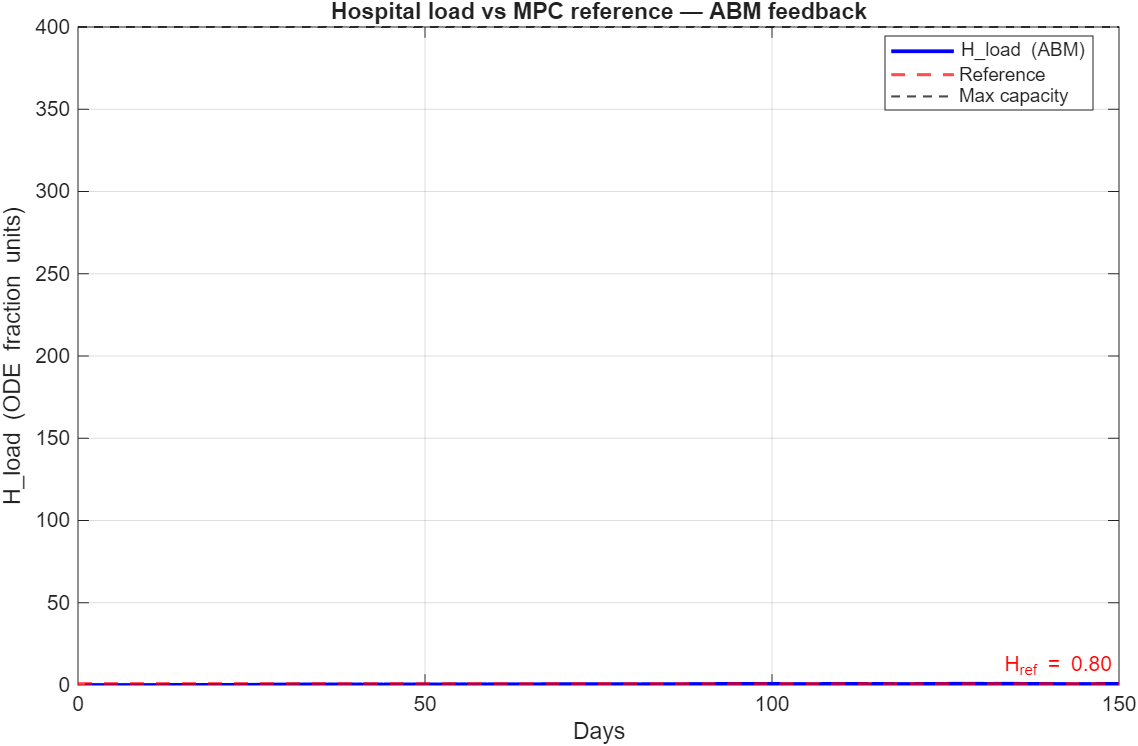
\includegraphics[width=0.85\textwidth]{Figures/jama/h_load_vs_reference_uploaded}
  \caption{%jama
    Hospital load under MPC control relative to the reference threshold $H_{\mathrm{ref}} = 0.8$
    (dashed line) used by the controller.
    The closed-loop trajectory remains close to the target level,
    indicating effective constraint handling at the micro level.}
  \label{fig:h_load_vs_ref}
\end{figure}

This result is significant because the MPC was designed and tuned entirely on the macro compartmental ODE model, with no knowledge of individual agent positions, travel decisions, or stochastic fluctuations.
The fact that its output successfully guides the stochastic micro simulation toward lower infection and hospitalisation counts demonstrates the robustness of the control design across model scales.
